\chapter{Literature Review}\label{ch:lit}

% ==================================================================
\section{Chapter overview}\label{sec:lit-overview}
% ==================================================================
This chapter critically reviews the knowledge on which \prism{} is built, spanning traffic engineering,
control theory, sensing, simulation and computer vision. Each strand is read with one question in mind: what does
it contribute to, or leave unsolved for, the control of a single junction carrying heterogeneous, weakly
lane-disciplined traffic such as that at Maviththara? Where a technique is judged unsuitable, the reasons are
stated; where it is adopted, the decision is justified.

\Cref{sec:lit-conceptmap} maps the literature, \cref{sec:lit-domain} overviews the domain,
\cref{sec:lit-existing} compares existing systems, \cref{sec:lit-tech} analyses algorithms, designs and
workflows, and \cref{sec:lit-reflection} justifies the research gap and design decisions. Foundational theory is
cited from its original sources; the state of the art concentrates on work from 2021 onwards.

% ==================================================================
\section{Conceptual map of the literature}\label{sec:lit-conceptmap}
% ==================================================================
\Cref{fig:lit-conceptmap} organises the literature around Adaptive Traffic Signal Control (ATSC), with five
branches: control strategies, sensing technologies, heterogeneous traffic and Passenger Car Units (PCU),
simulation and calibration, and computer vision for trajectory extraction. Bold items were adopted by this
research; the others were rejected or used as baselines, for the reasons given in \cref{sec:lit-reflection}.

\begin{figure}[htbp]
  \centering
  \resizebox{\textwidth}{!}{%
  \begin{tikzpicture}[
      font=\small,
      branch/.style={rectangle split, rectangle split parts=2, draw, rounded corners=2pt,
        text width=5.0cm, align=left, rectangle split part fill={black!10,white}, inner sep=3pt},
      hub/.style={ellipse, draw, very thick, fill=black!10, align=center, inner sep=3pt, font=\small\bfseries},
      link/.style={-{Latex[length=2.2mm]}, thick, black!70},
      flow/.style={dashed, black!60, -{Latex[length=2mm]}},
      lbl/.style={font=\footnotesize\itshape, align=center, text=black!70}]
    \node[hub] (c) at (0,0.4) {Adaptive traffic\\signal control\\(single junction)};
    \node[branch, anchor=north] (ctl) at (-5.6,5.6) {\textbf{Control strategies} (\S2.4, \S2.5.1)
      \nodepart{two}Fixed-time; \textbf{Webster (B3)}\\
      Actuated, gap-out (B2)\\
      Model-based adaptive: SCOOT, SCATS, OPAC, RHODES, SURTRAC\\
      \textbf{Max-pressure} and variants\\
      RL / deep RL};
    \node[branch, anchor=north] (sen) at (5.6,5.6) {\textbf{Sensing} (\S2.5.2)
      \nodepart{two}Inductive loops; video cameras; radar\\
      \textbf{Roadside LiDAR} (simulated as the \vls{})\\
      \textbf{Drone (UAV) video} for calibration};
    \node[branch, anchor=north] (pcu) at (-5.6,-1.4) {\textbf{Heterogeneous traffic} (\S2.3)
      \nodepart{two}Lane-less, mixed streams\\
      Motorcycles and three-wheelers\\
      \textbf{PCU weighting}, saturation flow};
    \node[branch, anchor=north] (sim) at (5.6,-1.4) {\textbf{Simulation \& calibration} (\S2.5.2)
      \nodepart{two}\textbf{SUMO + TraCI, sublane model}\\
      CARLA; VISSIM / Aimsun\\
      \textbf{GEH, MAPE} calibration targets};
    \node[branch, anchor=north] (vis) at (0,-4.6) {\textbf{Vision for data extraction} (\S2.5.1)
      \nodepart{two}Detection: \textbf{YOLOv8}, YOLO11, RT-DETR, Faster R-CNN\\
      Small objects: \textbf{SAHI} tiling\\
      Tracking: SORT, DeepSORT, \textbf{ByteTrack}};
    \draw[link] (c) -- (ctl);
    \draw[link] (c) -- (sen);
    \draw[link] (c) -- (pcu);
    \draw[link] (c) -- (sim);
    \draw[link] (c) -- (vis);
    \draw[flow] (pcu.north) -- node[lbl, right] {PCU weights\\pressure} (ctl.south);
    \draw[flow] (sen.south) -- node[lbl, left] {LiDAR objects\\feed state} (sim.north);
    \draw[flow] (vis.east) -| node[lbl, pos=0.3, below] {demand and calibration data} (sim.south);
  \end{tikzpicture}}
  \caption{Conceptual map of the literature reviewed in this chapter. Bold items were adopted by this research;
  dashed arrows show how the strands inform one another in \prism{}.}
  \label{fig:lit-conceptmap}
\end{figure}

% ==================================================================
\section{Domain overview}\label{sec:lit-domain}
% ==================================================================
A traffic signal allocates the right of way between conflicting streams in time rather than in space. A
\emph{movement} is a stream travelling from one approach to one exit; a \emph{phase} is a set of mutually
compatible movements that receive green together; and the \emph{cycle} of length $C$ is one complete sequence
of phases. Between consecutive greens an \emph{intergreen} (amber plus all-red) clears the junction; together
with the start-up delay of queued drivers it produces \emph{lost time} $L$ during which the junction discharges
nothing \cite{koonce2008timing}. The key capacity parameter is the \emph{saturation flow} $s$, the rate at which
a standing queue discharges once the start-up transient has passed. For a movement with arrival flow $q$ and
effective green $g$, capacity is $sg/C$ and the degree of saturation is $x=qC/(sg)$. The Highway Capacity
Manual (HCM) measures performance chiefly through \emph{control delay} \cite{hcm2016}, the basis of the metrics
in \cref{ch:eval}.

All of these formulations assume a homogeneous stream of ``standard'' cars travelling in lanes. Traffic in
Sri Lanka, as in much of South Asia, violates both assumptions. Motorcycles are the largest category of the
registered fleet and three-wheelers form another large share \cite{dmt_stats}; at the stop line these vehicles
weave between cars, travel two or three abreast within a single marked lane and accumulate ahead of larger
vehicles. The conventional remedy is to express flows in PCU, weighting each vehicle by its impact on capacity
relative to a passenger car \cite{irc106}. Recent South Asian studies show that PCU values at signalised
intersections are not constants but vary with composition, queue position and the share of two-wheelers
\cite{jatoth2023modeling,perera2025pce}, and that base saturation flow in non-lane-based traffic differs markedly
from Western defaults \cite{sugiarto2024base}. A 2026 systematic review of Sri Lankan junctions goes further,
reporting saturation flows of up to 2574~PCU/h/lane and arguing that motorcycle seepage, lateral filtering and
initial surge make static PCU factors and classical timing methods unreliable \cite{salawavidana2026why}. The author draws two conclusions from this literature. First, any controller that counts vehicles
rather than road-space demand will misjudge a queue of ten motorcycles against a queue of ten buses. Second,
because exact PCU values are context-dependent, a controller should treat them as tunable parameters derived
from local observation rather than as universal constants, which is the approach taken in this research using
the drone-derived saturation flow.

Institutionally, the Colombo metropolitan transport study documented growing congestion and called for better
traffic management \cite{jica2014comtrans}. Suburban junctions such as Maviththara run fixed-time plans, and in
severe congestion the police switch the signals off and direct traffic manually, which is labour-intensive,
inconsistent and hazardous for officers. The few recent local adaptive proposals rely on camera-based detection
\cite{wijesekara2025signals} or reinforcement learning \cite{shangeeth2025emission}, both of which raise
concerns examined in \cref{sec:lit-existing}.

% ==================================================================
\section{Existing systems, frameworks and designs}\label{sec:lit-existing}
% ==================================================================
\subsection{Fixed-time and vehicle-actuated control}
\emph{Fixed-time} control repeats a predetermined cycle, split and phase order, possibly with time-of-day plans.
It is cheap, predictable, independent of detectors and easy to coordinate along arterials
\cite{koonce2008timing}. Its weakness is that the plan is optimised for an assumed demand: when arrivals
deviate, green is wasted on empty approaches while queues grow elsewhere. Maviththara runs a 78~s, four-phase plan. \emph{Vehicle-actuated} control adds local feedback from detectors:
each phase runs between a minimum and a maximum green and is extended while vehicles keep arriving, ``gapping
out'' when the headway exceeds a threshold \cite{koonce2008timing,sumo_actuated}. In the author's assessment,
actuation helps at light and moderate demand but is myopic. It considers only the phase
being served and never compares competing queues, so under heavy demand every phase runs to its maximum and the
controller collapses into a fixed-time plan at maximum settings, precisely the morning-peak condition at
Maviththara.

\subsection{Model-based adaptive systems}
Model-based adaptive systems adjust timings continuously from measured demand
\cite{papageorgiou2003review,stevanovic2010nchrp}. \textbf{SCOOT} (Split, Cycle and Offset Optimisation
Technique) builds cyclic flow profiles from upstream loops and makes frequent small adjustments to splits,
offsets and cycle length to minimise a delay-and-stops index \cite{hunt1981scoot}. \textbf{SCATS} (Sydney
Coordinated Adaptive Traffic System) uses stop-line loops to compute a degree-of-saturation measure and adapts
cycle, splits and offsets hierarchically \cite{sims1980scats}. \textbf{OPAC} (Optimisation Policies for Adaptive
Control) \cite{gartner1983opac} and \textbf{RHODES} (Real-time Hierarchical Optimised Distributed Effective
System) \cite{mirchandani2001rhodes} drop the fixed cycle altogether and optimise switching times over a rolling
horizon from predicted arrivals. \textbf{SURTRAC} (Scalable Urban Traffic Control) treats each junction as a
real-time scheduling problem over clusters of approaching vehicles and coordinates neighbours by exchanging
predicted outflows \cite{xie2012surtrac}. A recent review of adaptive signal control describes these systems as the established practice against which
newer learning-based approaches are measured, and notes their dependence on fixed detector infrastructure
\cite{miletic2022review}.

The author regards these systems as the engineering benchmark but questions their transferability to a suburban
Sri Lankan junction for three reasons. First, they are proprietary, require central infrastructure and
specialist staff, and their cost and detector maintenance are recurrent concerns even in high-income agencies
\cite{stevanovic2010nchrp}. Second, they rely on inductive loops cut into the carriageway, which register
lane-following vehicles well but miss motorcycles filtering along lane edges. Third, their internal traffic
models assume lane-disciplined, predominantly four-wheeled flows; a loop occupancy says little about the true
PCU load of a queue in which motorcycles and three-wheelers fill every lateral gap.

\subsection{Max-pressure control and its deployments}
Max-pressure control, introduced to road traffic by Varaiya \cite{varaiya2013maxpressure} from the back-pressure
scheduling of communication networks \cite{tassiulas1992}, selects at each decision instant the phase whose
movements have the largest difference between upstream and downstream queues. It needs no demand forecast, is
decentralised, and is provably throughput-optimal under its modelling assumptions. Since 2021 the family has
matured from theory towards practice. The synthesis by Levin of methodological and experimental results
\cite{levin2023maxpressure} traces variants for cyclic phasing, realistic flow models, measurement error and
multiple modes, reports that calibrated simulations mostly favour max-pressure over existing timings, and notes
that field trials have begun; moreover,
corridor studies with realistic phasing have shown that cyclical max-pressure can outperform actuated
coordination in microsimulation of real networks \cite{barman2022performance}. Delay-based \cite{liu2022novel}
and switching-loss-aware \cite{wang2022learning} variants address two practical weaknesses of the original
policy, coordination-aware variants smooth platoons along corridors \cite{xu2024smoothingmp}, and a two-layer
scheme that combines max-pressure at critical nodes with perimeter control has been shown to remain effective in
a large network with finite queues and spillback \cite{tsitsokas2023twolayer}. The author finds this trajectory
persuasive: max-pressure offers a compact, auditable rule whose
behaviour can be explained to a traffic police officer, and its local information requirement matches what a
single pole-mounted sensor can provide. However, none of the reviewed max-pressure studies considered
lane-less, PCU-heterogeneous traffic or imperfect, sensor-derived queue estimates.

\subsection{Learning-based systems}
Reinforcement Learning (RL) frames signal control as a sequential decision problem, from early tabular
Q-learning at an isolated junction \cite{abdulhai2003rl} and multi-agent schemes \cite{arel2010rl} to Deep
Reinforcement Learning (DRL) agents trained on high-resolution vehicle positions \cite{genders2016drl} and
evaluated on real city data \cite{wei2018intellilight}. Recent surveys \cite{wei2021recent,noaeen2022rl,
haydari2022deep} report rapid progress in simulation, and pressure-aware state designs have become state of the
art in benchmarks \cite{zhang2022expression}. Yet the same surveys acknowledge that real-world deployments
remain rare and that evaluation is dominated by simulated, lane-disciplined scenarios; the most recent review
again names scalability, real-time adaptability and the sim-to-real gap as open problems \cite{xiao2025advances}.
Closer to the study site, a Sri Lankan RL controller \cite{shangeeth2025emission} and a camera-based adaptive
proposal for a Matara junction \cite{wijesekara2025signals} report gains in simulation, and an edge-deployed
YOLO-based controller weighting vehicles by passenger car equivalents has been proposed abroad \cite{raza2025edgeatlc}. The
author welcomes these as evidence of local interest, but notes that none was calibrated with observed
trajectories of the junction concerned, and that the camera-based designs inherit the night-time and privacy
weaknesses discussed in \cref{sec:lit-design}. The author's view is that
a policy whose decisions cannot be explained, which must be retrained when demand or geometry changes and which
offers no formal safety guarantee, is unlikely to be accepted by the Road Development Authority (RDA) or the
traffic police in the near term. Notably, the strongest RL designs now use pressure as a state feature, which
suggests that the explanatory power lies largely in the pressure concept itself.

\subsection{Comparative assessment}
\Cref{tab:lit-systems} compares the reviewed systems against criteria that matter for the study site.

\begin{table}[htbp]
\centering
\caption{Comparative assessment of existing signal control systems against the requirements of the study site.}
\label{tab:lit-systems}
\footnotesize\setlength{\tabcolsep}{3pt}\renewcommand{\arraystretch}{1.15}
\begin{tabularx}{\textwidth}{>{\raggedright\arraybackslash}p{1.9cm} >{\raggedright\arraybackslash}p{1.7cm}
  >{\raggedright\arraybackslash}p{2.1cm} >{\centering\arraybackslash}p{1.2cm} >{\centering\arraybackslash}p{1.25cm}
  >{\raggedright\arraybackslash}p{1.55cm} >{\raggedright\arraybackslash}X}
\toprule
System & Sensing & Decision method & Hetero.\ traffic aware & Explain\-able & Data needs & Main limitation for the study site \\
\midrule
Fixed-time / Webster \cite{webster1958} & None & Offline cycle and split optimisation & No & Yes & Historical counts & Cannot react to demand fluctuations \\
Actuated \cite{koonce2008timing} & Loops at stop line & Gap-out between min/max green & No & Yes & Low & Myopic; saturates to max green \\
SCOOT \cite{hunt1981scoot} & Upstream loops & Incremental split/offset/cycle optimisation & No & Partly & Dense loops, calibration & Proprietary, costly, lane-based \\
SCATS \cite{sims1980scats} & Stop-line loops & Degree-of-saturation plan selection & No & Partly & Dense loops & Proprietary; vehicle counts only \\
OPAC / RHODES \cite{gartner1983opac,mirchandani2001rhodes} & Upstream loops & Rolling-horizon optimisation & No & Partly & Arrival prediction & Computationally and data intensive \\
SURTRAC \cite{xie2012surtrac} & Loops, video & Real-time cluster scheduling & No & Partly & Approach-level detection & Commercial; lane-based clusters \\
Max-pressure \cite{varaiya2013maxpressure,levin2023maxpressure} & Queue detectors & Argmax of phase pressure & No (vehicle counts) & Yes & Local queues & Assumes perfect counts and homogeneous vehicles \\
Deep RL \cite{wei2021recent,noaeen2022rl} & Simulated full state & Learned policy & Rarely & No & Large training sets & Opaque; sim-to-real gap; no safety proof \\
\midrule
\prism{} (this work) & Roadside LiDAR (simulated) & PCU-weighted pressure with fairness & Yes & Yes & Local LiDAR objects & Evaluated in simulation only \\
\bottomrule
\end{tabularx}
\end{table}

The table reveals what the author regards as the crux of this review: the systems that are explainable and
cheap (fixed-time, actuated, max-pressure) are blind to vehicle heterogeneity, while the
systems that could in principle learn heterogeneity (RL) are neither explainable nor deployable. No reviewed
system is simultaneously heterogeneity-aware, explainable and low in data demand.

% ==================================================================
\section{Technological analysis}\label{sec:lit-tech}
% ==================================================================
\subsection{Algorithmic analysis}\label{sec:lit-algorithms}

\subsubsection{Webster's fixed-time optimisation}
Webster \cite{webster1958} derived the average delay per vehicle on an approach,
\begin{equation}
  d = \frac{C(1-\lambda)^2}{2(1-\lambda x)} + \frac{x^2}{2q(1-x)} - 0.65\left(\frac{C}{q^2}\right)^{1/3} x^{(2+5\lambda)},
  \label{eq:lit-webster-delay}
\end{equation}
where $\lambda=g/C$. Minimising total delay yields the optimal cycle length
\begin{equation}
  C_0 = \frac{1.5L + 5}{1 - Y},
  \label{eq:lit-webster-c0}
\end{equation}
with $Y=\sum_i q_i/s_i$ the sum of critical flow ratios, and greens shared as $g_i=(C_0-L)\,y_i/Y$
\cite{webster1958,koonce2008timing}. \Cref{fig:lit-webster} shows that $C_0$ grows without bound as $Y\to 1$.
The author draws a practical lesson from this curve: a fixed-time plan is most fragile exactly when demand is
highest, so even an optimally recomputed plan cannot absorb the minute-to-minute fluctuations of a morning peak.
Webster's method is nevertheless the fairest ``best fixed-time'' benchmark and is used as baseline B3.

\begin{figure}[htbp]
  \centering
  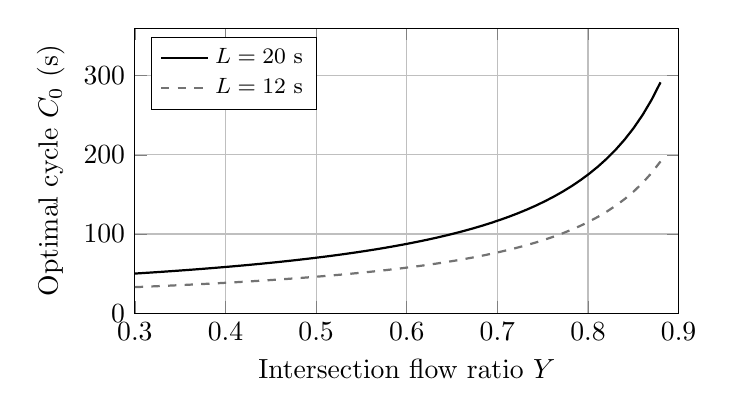
\begin{tikzpicture}
    \begin{axis}[width=0.70\textwidth,height=5.2cm,xlabel={Intersection flow ratio $Y$},
        ylabel={Optimal cycle $C_0$ (s)},xmin=0.3,xmax=0.9,ymin=0,ymax=360,grid=major,
        legend pos=north west,legend style={font=\footnotesize}]
      \addplot[thick,black,domain=0.3:0.88,samples=60]{(1.5*20+5)/(1-x)};
      \addlegendentry{$L=20$ s}
      \addplot[thick,dashed,black!55,domain=0.3:0.88,samples=60]{(1.5*12+5)/(1-x)};
      \addlegendentry{$L=12$ s}
    \end{axis}
  \end{tikzpicture}
  \caption{Webster's optimal cycle length (\cref{eq:lit-webster-c0}) against the intersection flow ratio.
  $L=20$~s corresponds to four phases with a 5~s intergreen each, as at the study site.}
  \label{fig:lit-webster}
\end{figure}

\subsubsection{Actuated gap-out logic}
Actuated control is an event-driven rule: after the minimum green, each detection resets a passage timer, and
the phase terminates when the timer expires (gap-out) or the maximum green is reached (max-out)
\cite{koonce2008timing}. SUMO's built-in implementation extends a phase while detected headways stay below a
configurable maximum gap within \texttt{minDur} and \texttt{maxDur} bounds \cite{sumo_actuated}, and forms
baseline B2 here. The gap-out idea is valuable and is retained in \prism{} as one of several termination rules;
what is rejected is the use of gap-out as the \emph{only} criterion, because it never weighs the cost of making
other queues wait.

\subsubsection{Max-pressure theory and variants}
Let $x_l(t)$ be the queue on link $l$, $r(l,m)$ the turning ratio and $c(l,m)$ the saturation flow of movement
$(l,m)$. Varaiya's movement weight and phase pressure are
\begin{equation}
  w_{l,m}(t) = x_l(t) - \sum_{p} r(m,p)\,x_m(t), \qquad
  P_j(t) = \sum_{(l,m)\in j} w_{l,m}(t)\,c(l,m),
  \label{eq:lit-mp}
\end{equation}
and the controller activates $j^\ast=\arg\max_j P_j(t)$ \cite{varaiya2013maxpressure}. Under a store-and-forward
queueing model this policy stabilises all queues whenever demand lies inside the capacity region, without
knowing the demand \cite{varaiya2013maxpressure,tassiulas1992}. Early extensions established distributed
implementations \cite{wongpiromsarn2012distributed}, simulated arterial performance \cite{kouvelas2014maxpressure}
and normalised queues by link capacity to avoid spillback \cite{gregoire2015capacity}. Position-weighted
back-pressure further weights vehicles by their distance to the stop line so that the state reflects vehicles
about to arrive \cite{li2019position}. Post-2021 work has targeted the gaps between theory and practice: the
original proof ignores the lost time incurred at every phase change, which motivated switching-loss-aware
formulations \cite{wang2022learning}; delay-based pressure replaces queue counts with accumulated delay to improve
fairness at low-demand approaches \cite{liu2022novel}; and cyclical variants preserve a fixed phase order that
drivers expect \cite{levin2023maxpressure,barman2022performance}.

From this literature the author identifies four assumptions that do not hold at Maviththara and that \prism{}
was designed to relax. (i) Queues are counted in vehicles, implicitly homogeneous. (ii) Phase changes are
treated as free, whereas each costs 5~s of intergreen. (iii) Queues on all links are assumed to be observed
exactly, whereas a real sensor has limited range, noise, dropout and occlusion. (iv) Stability is a long-run
property, so an approach with persistently low pressure can be starved in the short run. The variants above
each relax one of these assumptions; none relaxes all four together, and none addresses (i) at all.

\subsubsection{Reinforcement learning and its limits for deployment}
DRL controllers learn a mapping from a high-dimensional state to a phase choice by maximising cumulative reward
\cite{genders2016drl,wei2018intellilight}. Surveys published since 2021 converge on a common list of obstacles to
deployment: sample inefficiency and long training, sensitivity to reward design, poor transfer between
junctions and demand patterns, the sim-to-real gap, and the absence of safety guarantees, which must be imposed
by external constraint wrappers \cite{wei2021recent,haydari2022deep,noaeen2022rl,xiao2025advances}. Benchmarks also
show that well-tuned max-pressure remains a strong baseline that many published agents only marginally beat
\cite{wei2019survey,zhang2022expression}. The author therefore concludes that, for a single junction whose
controller must be approved and supervised by the RDA and the traffic police, the marginal gain RL might offer does not justify
its opacity and data demand. Hence the \prism{} control law is pure mathematics.

\subsubsection{Vehicle detection}
For the offline extraction of trajectories from drone video, object detection is required. Two-stage detectors
such as Faster R-CNN \cite{ren2015faster} propose and then classify regions, giving high accuracy at high cost.
Single-stage detectors descended from YOLO (You Only Look Once) \cite{redmon2016yolo} predict boxes in one pass;
a 2023 review traces the family from YOLOv1 to YOLOv8 and documents steady gains in the accuracy--speed trade-off
\cite{terven2023comprehensive}. YOLOv8 \cite{jocher2023yolov8} adopted an anchor-free head and a mature training
and export toolchain; YOLOv9 \cite{wang2024yolov9} and YOLOv10 \cite{wang2024yolov10} improved gradient flow and
removed non-maximum suppression respectively, and YOLO11 \cite{khanam2024yolov11} refined the backbone.
Transformer-based RT-DETR (Real-Time Detection Transformer) \cite{zhao2024rtdetr} also eliminates
non-maximum suppression with competitive real-time accuracy. The author notes that for offline processing of a
few hours of video, inference speed is secondary; what matters is accuracy on very small objects, availability
of aerial pre-trained weights and the cost of fine-tuning on a free cloud Graphics Processing Unit (GPU). The newer models offer only
incremental accuracy gains on generic benchmarks, whereas YOLOv8 has the widest ecosystem of VisDrone-trained
weights and tiling integrations.

\subsubsection{Small-object detection in aerial imagery}
From an altitude of about \est{90~m} a motorcycle spans roughly twenty pixels in a 4K frame, and down-sampling to the
network input size erases it. The VisDrone challenge results show that small and densely packed objects remain
the dominant source of error for aerial detectors \cite{cao2021visdrone,zhu2022visdrone}, and dedicated
small-object variants of YOLOv8 for UAV imagery report gains mainly by preserving high-resolution features
\cite{wang2023uavyolov8}. Slicing Aided Hyper Inference (SAHI) takes a model-agnostic route: it runs the
detector on overlapping tiles and merges the results \cite{akyon2022sahi}. The author prefers SAHI to an
architecturally modified network because it can be applied to a standard, well-supported model and its benefit
can be measured simply by switching it on and off.

\subsubsection{Multi-object tracking}
Tracking-by-detection links detections into trajectories. SORT combines a Kalman filter with Hungarian
assignment on box overlap \cite{bewley2016sort}; DeepSORT adds an appearance embedding \cite{wojke2017deepsort};
ByteTrack associates low-confidence boxes in a second stage, recovering partially occluded objects
\cite{zhang2022bytetrack}. Successors such as BoT-SORT \cite{aharon2022botsort}, StrongSORT
\cite{du2023strongsort} and OC-SORT \cite{cao2023observation} add camera-motion compensation, stronger appearance
models or observation-centric motion recovery. Performance is reported through Multiple Object Tracking Accuracy
(MOTA) \cite{bernardin2008clearmot} and the Identification F1 score (IDF1) \cite{ristani2016idf1}. In the author's assessment, appearance
features add little in a nadir view where same-class vehicles look almost identical from above, and camera
motion is better removed once by frame stabilisation. ByteTrack's motion-only, two-stage association therefore
matches the problem best. \Cref{tab:lit-detectors} summarises the candidates.

\begin{table}[htbp]
\centering
\caption{Comparison of candidate detectors and trackers for drone-based vehicle extraction.}
\label{tab:lit-detectors}
\footnotesize\renewcommand{\arraystretch}{1.15}
\begin{tabularx}{\textwidth}{>{\raggedright\arraybackslash}p{2.6cm} >{\raggedright\arraybackslash}p{2.4cm}
  >{\raggedright\arraybackslash}X >{\raggedright\arraybackslash}X}
\toprule
Method & Type & Strengths & Weaknesses for this task \\
\midrule
Faster R-CNN \cite{ren2015faster} & Two-stage detector & High accuracy, well understood & Slow on long 4K video; heavier fine-tuning \\
YOLOv8 \cite{jocher2023yolov8} & Single-stage, anchor-free & Mature toolchain, VisDrone weights, SAHI support & Small objects need tiling \\
YOLOv9, YOLOv10, YOLO11 \cite{wang2024yolov9,wang2024yolov10,khanam2024yolov11} & Single-stage & Incremental accuracy and latency gains & Fewer aerial pre-trained weights at time of work \\
RT-DETR \cite{zhao2024rtdetr} & Transformer & No non-maximum suppression; competitive accuracy & Higher training cost on a free GPU \\
\midrule
SORT \cite{bewley2016sort} & IoU + Kalman & Very fast, simple & Drops low-score boxes; identity switches \\
DeepSORT, StrongSORT \cite{wojke2017deepsort,du2023strongsort} & + appearance & Fewer switches in pedestrian scenes & Re-ID of little use for top-down vehicles \\
OC-SORT, BoT-SORT \cite{cao2023observation,aharon2022botsort} & Motion-centric / camera-motion compensation & Robust to occlusion and camera motion & Extra complexity once video is stabilised \\
ByteTrack \cite{zhang2022bytetrack} & Two-stage association & Keeps occluded, low-score objects; no Re-ID & Sensitive to detection thresholds \\
\bottomrule
\end{tabularx}
\end{table}

\subsection{Design analysis}\label{sec:lit-design}

\subsubsection{Sensing technologies}
\emph{Inductive loops} are accurate
for lane-following vehicles but intrusive, point-based and prone to missing small vehicles off the lane centre.
\emph{Video cameras} provide wide-area, classifiable data but degrade at night, in rain and under glare, and
capture identifiable faces and plates. \emph{Radar} is robust to weather and measures speed directly but has
limited resolution for closely spaced small vehicles. \emph{Roadside LiDAR} (Light Detection and Ranging)
measures three-dimensional geometry with an active laser, independently of ambient light. Early roadside
pipelines demonstrated detection, classification and tracking of road users \cite{zhao2019lidar,lv2019lidar},
and recent reviews of infrastructure-based LiDAR perception describe a maturing chain of background filtering,
clustering, classification and tracking, while identifying occlusion, sparse returns at range and adverse
weather as the main residual error sources \cite{sun2022object,bai2022infrastructure}. Studies since 2021
have derived turning counts, queue lengths, arrivals on green and pedestrian waits directly from LiDAR
trajectories at a signalised intersection, in real time rather than after days of aggregation
\cite{saldivarcarranza2024vehicle}.
\Cref{tab:lit-sensors} compares the options.

\begin{table}[htbp]
\centering
\caption{Qualitative comparison of traffic sensing technologies for junction control (synthesised from
\cite{koonce2008timing,zhao2019lidar,sun2022object,bai2022infrastructure,goodall2013cv}).}
\label{tab:lit-sensors}
\footnotesize\setlength{\tabcolsep}{3pt}\renewcommand{\arraystretch}{1.15}
\begin{tabularx}{\textwidth}{>{\raggedright\arraybackslash}p{2.2cm} *{5}{>{\raggedright\arraybackslash}X}}
\toprule
Criterion & Inductive loop & Video camera & Radar & Roadside LiDAR & Connected vehicles \\
\midrule
Capital cost & Low per loop, high installation & Low--medium & Medium & Medium--high (falling) & Low if fleet equipped \\
Coverage & Point & Wide area & Wide area & 360\textdegree{}, whole junction & Equipped vehicles only \\
Night / weather & Robust & Poor at night, in rain & Robust & Robust at night; moderate in heavy rain & Robust \\
Privacy & High & Low (identifiable) & High & High (no imagery) & Medium \\
Size / class & Weak & Good & Weak & Good (3-D extent) & Self-reported \\
Lane-less traffic & Poor & Good & Moderate & Good & Penetration-limited \\
Occlusion & None & High & Moderate & Moderate (tall vehicles) & None \\
\bottomrule
\end{tabularx}
\end{table}

For Maviththara the author judges LiDAR the most suitable choice: it works by day and night, records no
identifiable imagery, and its three-dimensional extent yields vehicle length, from which a size class and hence
a PCU weight follow without a learned classifier. Data reported by connected vehicles \cite{goodall2013cv} would avoid sensing
altogether but depends on market penetration, which is negligible in Sri Lanka. LiDAR's weaknesses (cost and
occlusion by buses and lorries) are acknowledged and are modelled explicitly in the \vls{}
(\cref{sec:impl-vls}) rather than assumed away.

\subsubsection{Simulation platforms}
Simulation of Urban MObility (SUMO) \cite{lopez2018sumo} is open source, multi-modal and controllable at every step through the
Traffic Control Interface (TraCI) \cite{wegener2008traci}. Its default Krau{\ss} car-following model
\cite{krauss1998} and lane-change model \cite{erdmann2015lanechange} are complemented by a \emph{sublane model}
that divides lanes into narrow strips so that motorcycles can travel abreast and filter to the stop line
\cite{sumo_sublane}. Field measurements of motorcycle lateral clearance while filtering \cite{promraksa2022lane}
give empirical guidance for its lateral parameters, and SUMO has recently been calibrated for heterogeneous
traffic in Khulna, Bangladesh \cite{chowdhury2024calibration} and at the Piliyandala junction itself, where
a Mean Absolute Percentage Error (MAPE) below 15\% and GEH below 5 were reached with locally defined vehicle types \cite{salawavidana2026aggregate}. CARLA \cite{dosovitskiy2017carla} offers physically rendered cameras and LiDAR but is
built for autonomous-vehicle research and is far too heavy for hour-long, multi-seed experiments. Commercial
VISSIM and Aimsun are powerful but licence-bound, conflicting with a reproducible, zero-cost tool chain. The author therefore chose SUMO and wrote a lightweight
analytical LiDAR model over its vehicle state, rather than rendering point clouds in CARLA.

\subsubsection{Drone datasets and data extraction}
Drones observe a whole junction from above without occlusion or roadside installation. The highD
\cite{krajewski2018highd} and pNEUMA \cite{barmpounakis2020pneuma} datasets demonstrated that aerial video yields
accurate trajectories, the latter in dense urban traffic with many powered two-wheelers. A systematic review of
UAV-based urban traffic monitoring \cite{butila2022urban} and newer datasets such as exiD \cite{moers2022exid} and
CitySim \cite{zheng2024citysim} show that drone trajectories are now an accepted basis for calibration and
digital twins. VisDrone \cite{zhu2022visdrone} supplies labelled aerial images whose tricycle classes resemble
Sri Lankan three-wheelers. The author notes that all of these datasets were recorded in Europe, North America
or China; none reflects Sri Lankan composition. Even the local SUMO calibration at Piliyandala relied on
roadside video aggregated to 15-minute counts and queues \cite{salawavidana2026aggregate}, which cannot follow
individual motorcycles through the junction. Local nadir footage processed into per-vehicle trajectories was
therefore required.

\subsubsection{Calibration practice}
A simulation is credible only if calibrated. The Federal Highway Administration (FHWA) toolbox
\cite{dowling2004toolbox} recommends the GEH statistic,
\begin{equation}
  \mathrm{GEH} = \sqrt{\frac{2(M-C)^2}{M+C}},
  \label{eq:lit-geh}
\end{equation}
with $\mathrm{GEH}<5$ for at least 85\% of counts, alongside error measures such as MAPE on travel or
waiting times. Studies of heterogeneous traffic show that default
car-following and lane-change parameters are inadequate and must be tuned to local behaviour
\cite{mathew2010calibration,chowdhury2024calibration,salawavidana2026aggregate}, while automated pipelines
now fit SUMO demand and signal programmes to observed counts \cite{harth2022automated}. The author adopts both a count criterion (GEH) and a behavioural criterion
(MAPE of waiting time), because matching counts alone does not prove that the model reproduces queues.

\subsection{Workflow analysis}\label{sec:lit-workflow}
The reviewed studies share a common workflow: collect traffic data, build and calibrate a simulation,
implement the controller, and evaluate it against baselines over several seeds. The author identifies four
recurring shortcomings in its execution. First, controllers are commonly fed the simulator's ground truth, so
reported gains omit the cost of imperfect sensing. Second, demand is often synthetic or generic rather than
observed at the studied junction. Third, heterogeneity is rarely carried through every stage: even studies
calibrated with mixed traffic often evaluate a controller that counts vehicles. Fourth, the baseline is
frequently a single untuned fixed-time plan, which inflates improvements. \Cref{ch:method} shows how this
research closed each shortcoming: drone-observed demand, an explicit sensor model, PCU throughout, and three
baselines plus an oracle-sensor variant.

% ==================================================================
\section{Reflection}\label{sec:lit-reflection}
% ==================================================================
\subsection{Research gap}
Linking the findings above, the author identifies the following gap, summarised in \cref{tab:lit-gap}.
\begin{enumerate}[leftmargin=*,itemsep=2pt]
  \item Model-based adaptive systems are effective but costly, loop-dependent and modelled on lane-disciplined,
        largely four-wheeled traffic (\cref{sec:lit-existing}).
  \item Max-pressure is simple, decentralised and provably stabilising, and its recent variants address
        switching loss, delay and cyclic order \cite{levin2023maxpressure,liu2022novel,wang2022learning}, yet no
        variant weights pressure by PCU or combines it with an explicit fairness bound and realistic sensor
        error.
  \item DRL achieves strong simulated results but remains opaque, data-hungry and rarely deployed
        \cite{wei2021recent,noaeen2022rl}.
  \item Roadside LiDAR perception is maturing \cite{sun2022object,bai2022infrastructure}, but its use as the
        \emph{sole} input to a signal controller, with its errors modelled explicitly, is little explored.
  \item Drone trajectory data are established for calibration \cite{butila2022urban,zheng2024citysim}, but have
        not been used to calibrate a simulation of a Sri Lankan junction for evaluating adaptive control; the
        only local SUMO calibration used aggregated roadside video and evaluated no controller
        \cite{salawavidana2026aggregate}.
\end{enumerate}

\begin{table}[htbp]
\centering
\caption{Feature comparison of representative works and this research
(\checkmark{} = addressed, $\sim$ = partially, $\times$ = not addressed, -- = not applicable).}
\label{tab:lit-gap}
\footnotesize\renewcommand{\arraystretch}{1.15}
\begin{tabularx}{\textwidth}{X c c c c c c}
\toprule
Work & \shortstack{PCU\\weighting} & \shortstack{LiDAR\\input} & \shortstack{No-ML\\control} & \shortstack{Fairness\\bound} & \shortstack{Drone\\calib.} & \shortstack{Sri Lankan\\context} \\
\midrule
SCOOT / SCATS \cite{hunt1981scoot,sims1980scats} & $\times$ & $\times$ & \checkmark & $\sim$ & $\times$ & $\times$ \\
OPAC / RHODES / SURTRAC \cite{gartner1983opac,mirchandani2001rhodes,xie2012surtrac} & $\times$ & $\times$ & \checkmark & $\sim$ & $\times$ & $\times$ \\
Max-pressure and variants \cite{varaiya2013maxpressure,liu2022novel,levin2023maxpressure} & $\times$ & $\times$ & \checkmark & $\sim$ & $\times$ & $\times$ \\
Deep RL \cite{wei2021recent,zhang2022expression} & $\times$ & $\times$ & $\times$ & $\times$ & $\times$ & $\times$ \\
Roadside LiDAR \cite{sun2022object,bai2022infrastructure} & $\sim$ & \checkmark & -- & -- & $\times$ & $\times$ \\
Heterogeneous PCU studies \cite{irc106,jatoth2023modeling,salawavidana2026why} & \checkmark & $\times$ & -- & -- & $\times$ & $\sim$ \\
Drone datasets \cite{barmpounakis2020pneuma,zheng2024citysim} & $\sim$ & $\times$ & -- & -- & \checkmark & $\times$ \\
\midrule
\textbf{This work (\prism{})} & \checkmark & \checkmark & \checkmark & \checkmark & \checkmark & \checkmark \\
\bottomrule
\end{tabularx}
\end{table}

\subsection{Justification of design decisions}
Each design decision of this research follows from the review.
\begin{itemize}[leftmargin=*,itemsep=2pt]
  \item \textbf{LiDAR over camera or loops.} LiDAR is the only option in \cref{tab:lit-sensors} that is
        simultaneously light-independent, privacy-preserving and able to measure vehicle size in lane-less
        traffic. Because a physical unit was unaffordable, it was simulated; to avoid the ground-truth fallacy
        noted in \cref{sec:lit-workflow}, its noise, dropout, occlusion and size confusion were modelled.
  \item \textbf{Max-pressure over RL.} Max-pressure is explainable, theoretically grounded and needs no training,
        which suits authorities that must approve and supervise the controller, whereas DRL's deployment
        obstacles remain unresolved. Its four unrealistic assumptions were relaxed explicitly: PCU weighting,
        variable green bounded by $G_{\min}$ and $G_{\max}$ with hysteresis, a perception tracker, and an
        urgency term with a starvation cap.
  \item \textbf{PCU weighting.} Vehicle counts misrepresent load where motorcycles and buses share a queue; PCU,
        with the saturation flow measured locally, converts LiDAR size classes into road-space demand.
  \item \textbf{Drone calibration.} Existing trajectory datasets do not represent Sri Lankan composition, and
        loops do not exist at the site; a nadir drone captures every vehicle, including filtering motorcycles,
        with legal approval and without identifying individuals.
  \item \textbf{YOLOv8, SAHI and ByteTrack.} The combination offers the most mature aerial ecosystem, a
        model-agnostic remedy for twenty-pixel motorcycles, and a tracker suited to look-alike vehicles seen from
        above.
  \item \textbf{SUMO with the sublane model.} It is open, scriptable through TraCI, light enough for many seeds
        and the only reviewed free simulator that represents motorcycles filtering abreast.
\end{itemize}

\subsection{Chapter summary}
The review established that lane-less, heterogeneous traffic invalidates vehicle-count models; that no
existing system is at once heterogeneity-aware, explainable and frugal in data; and that max-pressure, with its
assumptions of homogeneous vehicles, free switching, perfect observation and implicit fairness relaxed, is the
most suitable control foundation. Roadside LiDAR, SUMO with its sublane model, and YOLOv8 with SAHI and
ByteTrack were selected as sensor, platform and extraction chain. \Cref{ch:method} operationalises these
decisions.
